\title{\textbf{Comparison throughput in Legacy and SDN networks using three types of TCP congestion algorithms}}
\author{\textbf{ Claudio Rimensi}\\University of Padua,\\Wireless Network} 
\maketitle
\begin{abstract}
{\emph{\footnotesize As organizations continue to the search for ways to accelerate time to increase revenue, reduce operational costs, and deploy new services at web speeds, Software-Defined Networking (SDN) is a fast emerging technology and shift in the traditional trappings of network design.SDN provides organizations accelerated application deployment and delivery, reduced IT costs, improved value of data center virtualization, increased resource flexibility, and greater cloud integration.   As computing trends continue to drive network change, SDN solves the challenges associated with networks that are ill-suited to the dynamic technology needs of today’s data centers.\\In this paper I would like to compare the throughput in a legacy and SDN networks using 3 different TCP congestion algorithms: TCP New-reno , TCP Vegas. and TCP Westwood.To create the legacy network I will use a simulation software called Network Simulator 2, while for the SDN network I will use Mininet to emulate the network and Onos as its controller.}}
\end{abstract}
\section{\normalsize Introduction}
{SDN stands for Software Defined Networking. It is an approach to networking that uses open protocols like OpenFlow to control software at the edge of the network. It is used to control access to switches and routers. It is nearly impossible to find a collective definition of SDN as its architecture can vary considerably from one organization to the next.\\ However, the basic purpose of SDN is to allow users to virtualize their hardware. A software-defined network attempts to build a computer network by separating it into two segments. The control plane is generally used to manage configurations of devices connected to the SDN on a remote basis.\\The second segment is the data plane which is responsible for forwarding traffic to its final destination. The control plane dictates which path flows will take before they reach the data plane. This is done through the use of a flow protocol. This segment is where an administrator interacts with the SDN and actually manages the network.
\subsection{\normalsize Different between SDN and legacy}{The biggest difference between a traditional network and SDN is that the latter is a software-based network. Traditional networks rely on physical infrastructure such as switches and routers to make connections and run properly. In contrast, a software-based network allows the user to control the allocation of resources at a virtual level through the control plane. Rather than interacting with physical infrastructure, the user is interacting with software to provision new devices.
\\
From this perspective, an administrator can ascertain network paths and actively configure network services. An SDN also has more ability to communicate with devices throughout the network than a traditional switch. The core difference between the two can be summed up as virtualization. SDN virtualizes your entire network. Virtualization creates an abstract version of your physical network which allows resources to be provisioned from a centralized location.
\\
The reason why SDN has become an alternative is that it allows administrators to provision resources and bandwidth instantaneously. It does so while eliminating the requirement to invest in more physical infrastructure. In contrast, a traditional network would need new hardware if its network capacity was to increase. The traditional model is to buy more equipment, not to press a button on a screen. The figure1 shows the different architeture of SDN and legacy apporach.
}
The rest of the paper is built as follows as:
Section2 related work. The section 3 and 4 will dedicate to explain the congestion control mechanism and the TCP congestion algortihms used in this experiment. In the section 5 I present the tools used to realize the proof and finally in the section 6 implementation in the real environment and tests.
\\\\\\\\\\\\\\\
\begin{figure}[!htb]
	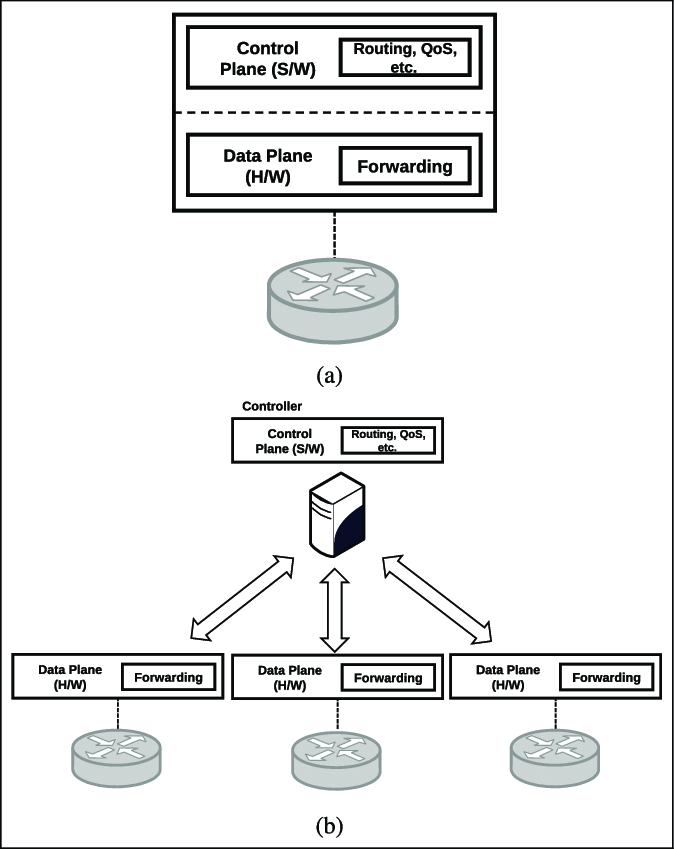
\includegraphics[width=7.6cm,height=9.0cm]{figura1}
	 \caption{Comparison between (b) SDN and (a) legacy architecture}
	\label{figure}
\end{figure}
}
\section{\normalsize Related Work}{
In this section, we just summarize the some of the relevant works about SDN and Legacy Networks with TCP congestion algorithms.
\begin{itemize}
\item In \cite{aa}  is presented an apporach that enables controller to select a long-lived flow to reduce sending rate by adjusting the TCP receive window of ACK packet after OpenFlow-switch triggered a congestion message to controller. The key benefit of SDTCP is that, with global perspective, we can accurately decelerate the rate of long-lived flow to ensure the performance other flows. The experiments indicate that we can achieve almost zero packet loss for TCP incast and guarantee goodput for the high propriety flows.
\item in \cite{bb} In this document, SDN technology is invoked to leverage large scale test benches to conduct end-to-end MPTCP experiments. More specifically, a special purpose control and measurement system is established in addition to two separate Internet test stands. First, using GÉANT's OpenFlow support, a test bed is built that allows measurements with real traffic. Second, a publicly available multipath measurement framework is designed on PlanetLab Europe and the challenges of such a system are shown. In addition, the results of MPTCP measurements in both test benches are presented to obtain information on its behaviour in an untested environment.
\item In \cite{cc} the paper proposes the flow congestion avoidance algorithm controlled by the network in SDN(Software Defined Networking) environment. In the proposed scheme, link utilization is calculated in SDN controller and recalculated rerouting algorithm is applied to switches which would be configured by using Openflow configuration protocol. To verify the improved performance, a video stream is applied to the proposed algorithm in SDN environment.
\item In \cite {dd} the NS-2 TCP-Linux project is explained. A preliminary assessment of three aspects of NS-2 TCP-Linux is also presented: extensibility to new congestion control algorithms, accuracy of simulation results and simulation performance in terms of simulation speed and memory usage. Based on these results, NS-2 TCP-Linux is a promising alternative or even a replacement for existing TCP implementations in NS-2. Participation is required to test and improve this new TCP implementation.
\item In \cite{ee} was carried out performance study of six variants of TCP to be able to classify which variant of TCP performs better in various possible scenarios in MANETs.
\item Finally in \cite{ff} End-to-end bandwidth estimation tools like Iperf though fairly accurate are intrusive. In this paper, was described how with an instrumented TCP stack (Web100), it was estimated the end-to-end bandwidth accurately, while consuming significantly less network bandwidth and time. It was modified Iperf to use Web100 to detect the end of slow-start and estimate the end-toend bandwidth by measuring the amount of data sent for a short period (1 second) after the slow-start, when the TCP throughput is relatively stable. It was obtained bandwidth estimates differing by less than 10 percent when compared to running Iperf for 20 seconds, and savings in bandwidth estimation time of up to 94 percent and savings in network traffic of up to 92%
\end{itemize}
}
\section{\normalsize Congestion Control Mechanisms}{
The TCP protocol presents a contrl functionality that allows to limit the amount of data transmitted in the form of packets and not yet encountered by the sender, adapting the data stream sent to the possible state the congestion of the network. This state is derived indirectly from information obtained from the state of the packet transmission by a terminal, thus avoiding congestion in the network itself.\\
The congestion control algorithm has two phases:
\begin{itemize}
	\item  Slow Start 
	\item Additive Increase Multiplicative Decrease (AIMD)
\end{itemize}
To distinguish between the two phases, a variable called ssthresh (slow start threshold) is used. When the value of the cwnd is less than the value of ssthresh we find ourselves in the slow start phase, otherwise we are in the AIMD phase. At the start of the transmission the variable is set to a very high value, while the size of the cwnd is equal to the size of a segment.
\subsection{\normalsize Slow Start}{
During the slow start phase the TCP sender starts transmitting the first data segment and waits for a reply. The congestion window cwnd increases by an amount equal to the MSS for each segment which, after being transmitted, is detected (an ACK is received). So at each RTT the cwnd doubles in size.\\
The slow start phase is maintained until a congestion event occurs, such as the loss of a data segment, or when the congestion window size reaches or exceeds the value of the ssthresh variable , event leading to the increase phase AIMD, or finally in the case in which three duplicated segments are identified.\\
Then we move on to the Congestion Avoidance algorithm when \textbf{(cwnd> = ssthresh)} or \textbf{ Fast retransmit} (when we identify three duplicate segments found).}
\subsection{\normalsize AIMD}{
Using the AIMD phase there is a linear additive increase of the cwnd value of 1 MSS each RTT . This can be achieved through the increase by the sender of his own cwnd of a quantity of bytes equal to:
\textbf{MSS * (MSS / cwnd)}, every time a new reply arrives. This behavior is called Additive Increase or Congestion Avoidance . The term Multiplicative Decrease refers to the behavior implemented by the sender upon receipt of three consecutive duplicate ACKs (with the same acknowledgment number): the variant TCP Reno, in this circumstance, sets the value of \textbf{SSTRESH} to \textbf{cwnd / 2} and assigns to cwnd this value increased by 3 MSS.\\ If the congestion becomes excessive, one or more buffers of routers along the path overflow, causing the deletion of an IP datagram that contains a TCP segment. Once this event has been detected at the end of a retransmission timeout, TCP reacts by halving the value of ssthresh and resetting cwnd to the size of a segment, thus returning to the slow start phase.
}
\subsection{\normalsize Fast Retransmit and Fast Recovery}{
The mechanisms described so far were part of the original proposal to add congestion control to TCP. It was soon discovered, however, that the coarse-grained implementation of TCP timeouts led to long periods of time during which the connection went dead while waiting for a timer to expire. Because of this, a new mechanism called fast re- transmit was added to TCP. Fast retransmit is a heuristic that sometimes triggers the retransmission of a dropped packet sooner than the regular timeout mechanism.
}

\section{\normalsize Variants of TCP}{
The three types of congestion algorithms used in this paper are TCP Vegas , TCP New-Reno and TCP Westwood:
\subsection{\normalsize TCP Vegas}{
TCP Vegas is a TCP algorithm that emphasizes packet delay rather than loss as a signal to determine the speed at which packets are sent from S to R.\\ 
The dynamics of the transmission window are based on a
throughput estimation obtained as follows:
\begin{itemize}
\item  Expected= Windowsize/BaseRTT, where BaseRTT is the minimum RTT value found.
\item For each segment is measured RTT and the number of bytes transmitted in that time. Define two threshold values $\alpha,\beta$:\\\\1) If the difference between the expected throughput and the calculated throughput is less than $\alpha$ linearly increases the cwnd window in the RTT next.\\\\2) If the difference is greater than $\beta$ cwnd it is decreased linearly in the next RTT
\item Slow start modified: tries to locate the correct value of the window without incurring a loss:\\\\1)When the current throughput is lower than the expected throughput, it is
go from slowstart to congestion avoidance
\item The retransmission takes place after a duplicate ack if the estimate of RTT is higher than the value of the time out.
\end{itemize}
}
\subsection{\normalsize TCP New-Reno}{
\begin{figure}[!htb]
	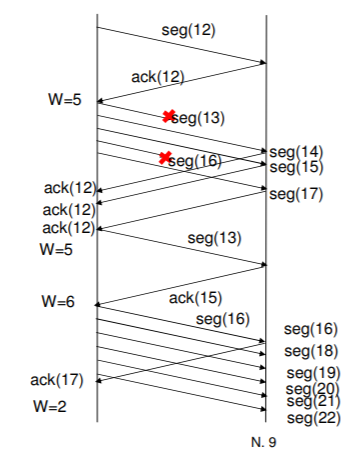
\includegraphics[width=7.6cm,height=9.0cm]{figure2}
	\caption{TCP New-Reno}
	\label{figure}
\end{figure}
The figure 2 shows how does TCP New-Reno works:	
\begin{itemize}
\item The first 12 segments were transmitted and recognized
\item Segment 13 and segment 16 are lost
\item The recognition of the loss of segment 13 occurs for 3  ack(12) duplicates.  The threshold is placed at 2, the window at 5
\item  Segment 13 is retransmitted. fast and triggers sending ack(15)
\item You don't get out of fast recovery, as in TCP Reno, because it's a partial ack. It is transmitted on 16 with
6 window and also 18,19,20,21,22.
\item Arrival ack(17) and departure in CA with window 2
\end{itemize}	
}
\subsection{\normalsize TCP Westwood}{
TCP Westwood is an end-to-end protocol. The sender is aware of the wireless knowledge.
Objectives:
\begin{itemize}
\item TCP Westwood tries to understand the difference between wireless errors and congestion errors and avoid that with the former the transmission speed slows down.
\item It involves changes only to the high sender of the connection. Useful for satellite communication.
\item Flow control is based on an estimate of the permissible bandwidth (BWE). Monitoring of ACKs on the transmitting side.
\item Event 3 duplicate ACKs:\\
SSTHRESH=BWE*RTTmin\\
if cwnd > SSTHRESH then cwnd=SSTHRESH
\item Event Timeout:\\
SSTHRESH=BWE*RTTmin
cwnd=1.
\end{itemize}
\textbf{Pro:}\\
1) Estimation of the bandwidth made by the sender side.\\
2) Code changes only on the sender side.\\
\textbf{Cons:}\\
1) Incorrect bandwidth estimation on asymmetric links.\\
2) Problems of correctness.\\
3) No specific mechanism to manage disconnections.\\

}
}
\section{\normalsize Description of the environment}{	
In this section I explain the description the tools and network topology used for my experiment.
\subsection{Tools used}{
For this experiment I used some tools.\\\\Concerning the Legacy Network I used the emulator called Ns2, while in the SDN network I used the simulator Mininet with the controller Onos.\\Also, in order to get the throughput and time results and represent them on the graph, I had to build some scripts that allowed me to do this.\\
\subsubsection{The simulator Ns2}{
NS version 2 is an event driven network simulator developed at UC Berkeley that simulates variety of IP networks. It implements network protocols such as TCP and UPD, traffic source behavior such as FTP, Telnet, Web, CBR and VBR, router queue management mechanism such as Drop Tail, RED and CBQ, routing algorithms such as Dijkstra, and more. NS also implements multicasting and some of the MAC layer protocols for LAN simulations.\\\\
\begin{figure}[!htb]
	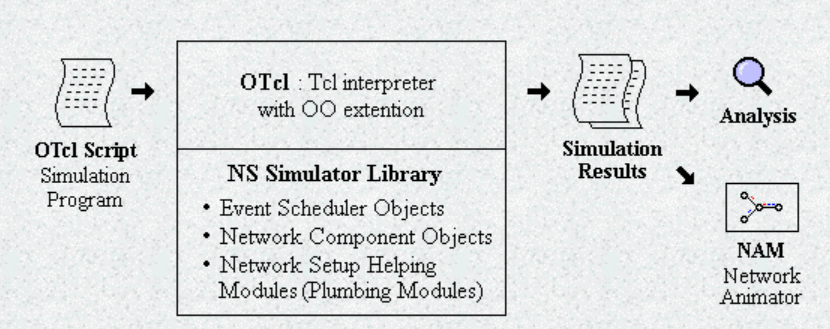
\includegraphics[width=7.6cm,height=4.0cm]{figura4}
	\caption{Simplified User's View of NS}
	\label{figure}
\end{figure}As shown in Figure 1, in a simplified user's view, NS is Object-oriented Tcl (OTcl) script interpreter that has a simulation event scheduler and network component object libraries, and network setup (plumbing) module libraries (actually, plumbing modules are implemented as member functions of the base simulator object).  The term "plumbing" is used for a network setup.
Another major component of NS beside network objects is the event scheduler. In NS, an event scheduler keeps track of simulation time and fires all the events in the event queue scheduled for the current time by invoking appropriate network components, which usually are the ones who issued the events, and let them do the appropriate action associated with packet pointed by the event. Network components communicate with one another passing packets. Another use of an event scheduler is timer. For example, TCP needs a timer to keep track of a packet transmission time out for retransmission (transmission of a packet with the same TCP packet number but different NS packet ID). 

}
\subsubsection{Mininet and Onos}{
Mininet provides a virtual test bed and development environment for software-defined networks (SDN). Mininet enables SDN development on any laptop or PC, and SDN designs can move seamlessly between Mininet (allowing inexpensive and streamlined development), and the real hardware running at line rate in live deployments. Mininet enables
\begin{itemize}
\item Rapid prototyping of software-defined networks
\item Complex topology testing without the need to wire up a physical network
\item Multiple concurrent developers to work independently on the same topology
\end{itemize}
Mininet networks run real code including standard Unix/Linux network applications as well as the real Linux kernel and network stack.
Mininet provides an extensible Python API for network creation and experimentations. It is released under a permissive BSD Open Source license and is actively developed and supported by community of networking and SDN enthusiasts.\\\\
ONOS stands for Open Network Operating System. ONOS provides the control plane for a software-defined network (SDN), managing network components, such as switches and links, and running software programs or modules to provide communication services to end hosts and neighboring networks.\\The most important benefit of an operating system is that it provides a useful and usable platform for software programs designed for a particular application or use case. ONOS applications and use cases often consist of customized communication routing, management, or monitoring services for software-defined networks. Some examples of things which you can do with ONOS, and software written to run on ONOS, may be found in Apps and Use Cases.
}
\subsubsection{Other tools}{
In order to get the information from the TCP congestion algorithms I used three other programs.\\\\
The first program, written in bash, creates the graph using the tool called gnuplot.\\The second program gives me the throughput in the network topology. Given the file (name.tr) that is the output of the script (name.tcl), it creates a file with two columns.  The first column shows all the instants of time ranging from 0 to 100 seconds while the second column shows me at every moment how throughput is. This file, written in perl, has some incoming arguments that are precisely the file (name.tr), the recipient node and every how often measure the throughput within the interval [0,100]s.\\ Finally, the last file is a script written in Python that automatically starts the server for me to run Onos. Once the server is ready, through a user-friendly menu, activate both the Onos Cli and its GUI. In the first active two applications of Onos, which are org.onosproject.fwd and org.onosproject.openflow, which allow me to let the hosts communicate with each other, while in the GUI I can see visually the network topology created. }
}
\subsection{Description of Network topology}{
	The figure 3 shows the network topology used from this experiment.
	\begin{itemize} 
		\item It is composed by 5 nodes. Node 0,Node 1,Node 2,Node 3, Node 4 and Node 5. 
		\item Node 0 and Node 1 communicate with Node 2, while Node 4 and 5 communicate with Node 3.All of this using duplex-link.
		\item For each link of communication there is a particular delay.
		\item I built this topology with\\ \textbf{bandwidth=10Mbits}.
		\item Between node 2 and node 3 there is an\\ \textbf{error= 0.01}.
		\item For this experiment I have decided to test the communication from node 0 to node 4 and node 1 to node5.
		\item The first route(node0-node4) has fewer delays than the second route(node1-node5) path. 
	\end{itemize}
}
\begin{figure}[!htb]
	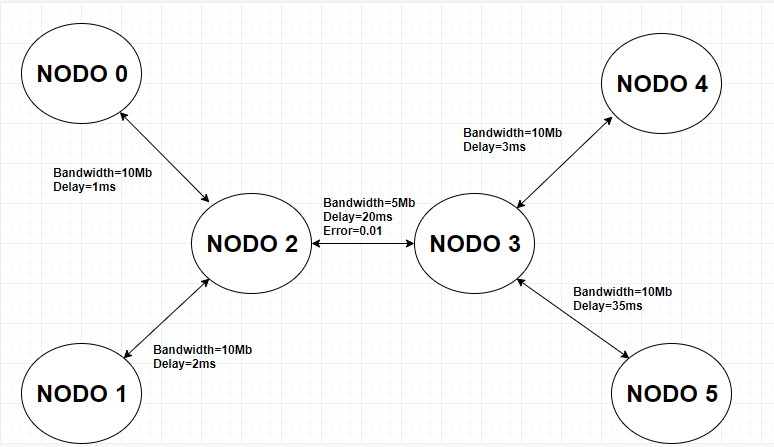
\includegraphics[width=7.6cm,height=6.0cm]{figura3}
	\caption{Network Topology with bandwidth and delay}
	\label{figure}
\end{figure}
}
\section{\normalsize Implementation and Result}{
In this section will be discuss the implementation of the network topology on the Ns2 and Mininet e the discuss of the results. The experiment is divided up in to 4 parts:
\begin {itemize}
\item Analyze, in Legacy environment, the behaviour of TCP New-Reno, TCP Vegas and TCP Westwood in the path from node 0 to node 4.
\item Analyze, in Legacy environment, the behaviour of TCP New-Reno, TCP Vegas and TCP Westwood in the path from node 1 to node 5.
\item Analyze, in SDN environment, the behaviour of TCP New-Reno, TCP Vegas and TCP Westwood in the path from node 0 to node 4.
\item Analyze, in SDN environment, the behaviour of TCP New-Reno, TCP Vegas and TCP Westwood in the path from node 1 to node 5.
\end{itemize}
\subsection{Implementation on Ns2}
{The simulation experiment is carried out in Linux (Ubuntu 18.04). The detailed simulation model is based on network simulator-2 (ver-2.31) \cite{hh}, is used in the evaluation. The NS instructions can be used to define the topology structure of the network and the motion mode of the nodes, to configure the service source and the receiver, to create the statistical data track file and so on.\\
Here below, I report a piece of code of my script, written in tcl, where I change the TCP congestion algorithms.\\
\begin{lstlisting}[frame=single,basicstyle=\small]
#Add a TCP sending module to node n0
set tcp [new Agent/TCP/Vegas]
#$ns at 0 "$tcp select_ca westwood"
$ns attach-agent $n0 $tcp

# Add a TCP receiving module to node n4
set sink1 [new Agent/TCPSink]
$ns attach-agent $n4 $sink1
...
$ns  trace-queue  $n3  $n4  $trace_file
\end{lstlisting}
This part of code is divided up in three parts:
\begin{itemize}
\item The part where I add TCP to the trasmittor node. In this case node 0. In the line of code \begin{lstlisting}[frame=single,basicstyle=\small]
set tcp [new Agent/TCP/Vegas]
\end{lstlisting} I can choose whether to use the congestion algorithms offered by NS2 or to use those on Linux. However, the Westwood congestion algorithm is not present on Ns2, so I had to use the one on Linux,using the instruction\begin{lstlisting}[frame=single,basicstyle=\small]
$ns at 0 "$tcp select_ca westwood" \end{lstlisting}

\item For the receiver I set TCP Sink which allows it to send ACKs once it has received the packet.
\item The last line of code I reported makes sure to keep track of the queue between node 3 and node 4. If instead the experiment was on the other path or between node 1 and node 5 I would have kept track of the queue between node 3 and node 5. 
\end{itemize}
}
\subsection{Implementation on Mininet}{
The simulation experiment is carried out in Linux (Ubuntu 18.04).\\As I said in section 5.1.3 below I started the controller Onos through the program I wrote in python, and then I started the network topology with the Mininet emulator. From the Mininet console I started two terminals with the xterm command. These terminals corresponded to the transmitter and receiver. First I tested the path from node 0 to node 4 and then from node 1 to node 5,using the tool iperf \cite{gg}.  
Specific instructions are given below.
\begin{lstlisting}[frame=single,basicstyle=\tiny]
#For the receiver node
iperf -s h4 or h5 -p 20
#For the transmitter node
sysctl net.ipv4.tcp_available_congestion_control= reno
iperf -c 10.0.0.4 or 10.0.0.5 -p 20 -i 1 -t 30 > result
cat result | grep sec | head -10 
| tr - " " |awk '{print $4,$8}'> newres
\end{lstlisting}

The receiver node, I set it with the command iperf as a server on port 20.
With regard to the client i.e. the transmitter, I proceeded in this way:
\begin{itemize}
	\item First I set the type of TCP congestion algorithm (reno,westwood,vegas).
	\item Through iperf I set the node as client and give it the IP of the server on port 20,and every second for a time of 30 seconds I measured the thorughput. 
	\item The measures ended up on the file called result. 
	\item The result file, however, had other writings over time and throughput, so I deleted them with this command \begin{lstlisting}[frame=single,basicstyle=\small]
cat result | grep sec | head -10 
|tr - " "|awk '{print $4,$8}'> newres 
	\end{lstlisting} 
	and the final result was redirected to the file called newres.
\end{itemize}
}
\subsection{Results}{
The throughput and time results for both the SDN and legacy architecture were then put as input to the program that later created the graphs using the gnuplot tool, as described in subsection 5.1.3.\\\\
Below here I report the graph about the path from node 0 to node 4 and from node1 to node 5 in SDN and Legacy network.
\begin{figure}[!htb]
	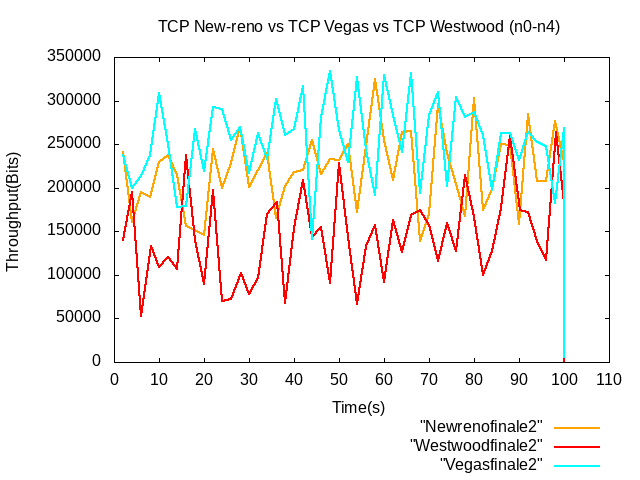
\includegraphics[width=7.6cm,height=6.0cm]{Legacy_n0-n4}
	\caption{Throughput in the Legacy network (n0-n4)}
	\label{figure}
\end{figure}
\begin{figure}[!htb]
	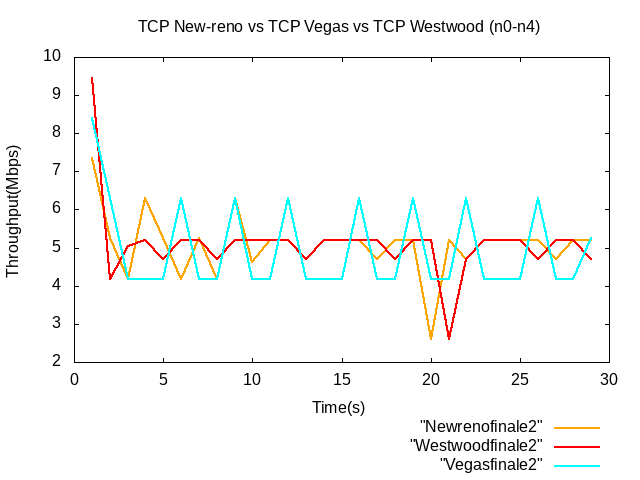
\includegraphics[width=7.6cm,height=6.0cm]{SDN_n0-n4}
	\caption{ Throughput in the SDN network (n0-n4)}
	\label{figure}
\end{figure}
\\\\\\
\begin{figure}[!htb]
	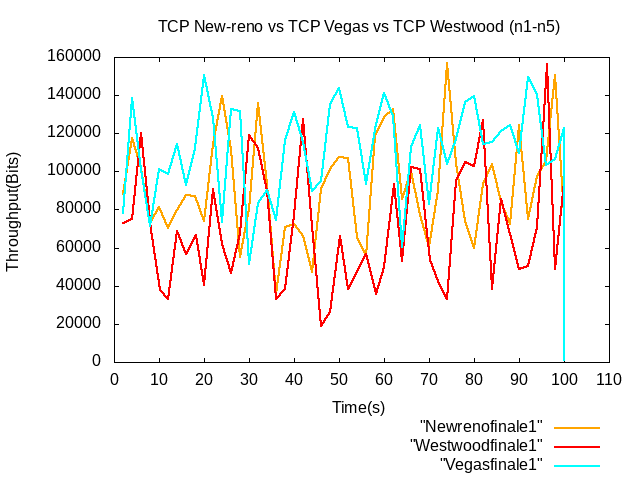
\includegraphics[width=7.6cm,height=6.0cm]{Legacy_n1-n5}
	\caption{Throughput in the Legacy network (n1-n5)}
	\label{figure}
\end{figure}
\\\\\\\
\begin{figure}[!htb]
	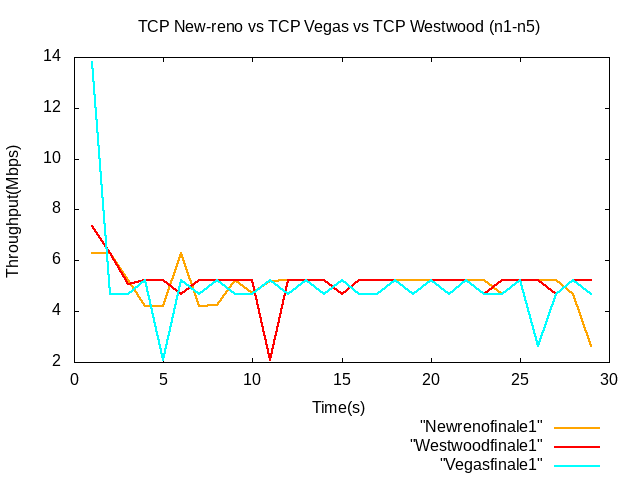
\includegraphics[width=7.6cm,height=6.0cm]{SDN_n1-n5}
	\caption{Throughput in the SDN network (n1-n5)}
	\label{figure}
\end{figure}
}
}
